% small.tex
\documentclass[handout]{beamer}
\usetheme{default}
\usepackage{color}
\usepackage[labelformat=empty]{caption}
\usepackage{amsfonts, amsmath, amsthm, amssymb,epstopdf}

%%% allows color text:
\usepackage{xcolor}

%%% Allows adding "links", i.e url
\usepackage{hyperref}

%\useoutertheme[subsection=false]{smoothbars}
\usetheme{Warsaw}
%\usecolortheme[rgb={0.2,0.3,0.7}]{structure}
%\setbeamercovered{highly dynamic}

\usepackage{amsmath,amssymb,latexsym}

%%% New commands:
\newcommand\independent{\protect\mathpalette{\protect\independenT}{\perp}} 

\theoremstyle{definition}
\newtheorem{defn}{Definition}[section]

% adding slide numbers
\addtobeamertemplate{navigation symbols}{}{%
    \usebeamerfont{footline}%
    \usebeamercolor[fg]{footline}%
    \hspace{1em}%
    \insertframenumber/\inserttotalframenumber
}
%%%%%%%%%%%%%%%%%%%%%%%%%%%%%%%%%%%%%%%%%%%%%%%%%%

\usepackage[round,sort,longnamesfirst]{natbib}

%%% Details:
\author{Yotam Shem-Tov}
\title{STAT 239/ PS 236A}

\begin{document}
\setbeamertemplate{caption}{\insertcaption}


\begin{frame}{}

\centering

\LARGE

$\bold{Section}$ $\bold{2:}$ $\bold{Introduction}$ $\bold{to}$ $\bold{potential}$ $\bold{outcome}$ $\bold{and}$ $\bold{causal}$ $\bold{relationships}$ \\~\\
$\bold{(and}$ $\bold{Monte-Carlo}$ $\bold{simulations})$

\vspace{0.4 in}

\large
\textit{Yotam Shem-Tov}

\vspace{0.1 in}

\textit{Fall 2014}

\end{frame}

%%%%%%%%%%%%%%%%%%%%%%%%%%%%%%%%
%%% Slides: 
%%%%%%%%%%%%%%%%%%%%%%%%%%%%%%%%


\begin{frame}{Definitions}
\begin{itemize}
\item Let $T_i$ be an indicator variable whether individual $i$ received treatment ($T_i=1$) or control ($T_i=0$)
\item Let $Y_{i1}$ be the potential outcome of individual $i$ with treatment and $Y_{i0}$ the potential outcome without treatment
\item The observed outcomes are,
$$Y_i = T_i Y_i1 +(1-T_i)Y_{i0}$$
\pause
	\small
		 \begin{tabular}{ccc}
		\hline
		Group & $Y_{i1}$ & $Y_{i0}$\\
		\hline
		 $T=1$ & Observable: $Y_{i1}|T=1$ & Counterfactual: $Y_{i0}|T=1$\\
		 $T=0$ & Counterfactual: $Y_{i1}|T=0$ & Observable: $Y_{i0}|T=0$\\
		\hline
		\end{tabular}
	\normalsize
\end{itemize}
\end{frame}

\begin{frame}
\begin{itemize}
\item The treatment effect on individual $i$ is,
$$ \tau_i = Y_{i1} - Y_{i0}$$ 
\pause
\item There can be many parameters of interest. A few common parameters are,
$$ATE = \mathbb{E}\left(Y_{i1} - Y_{i0} \right)$$
$$ATT = \mathbb{E}\left(Y_{i1} - Y_{i0}| T_i=1 \right)$$
$$ATC = \mathbb{E}\left(Y_{i1} - Y_{i0}| T_i=0 \right)$$
\pause
\item We can also be interested in the treatment effect conditional on a certain value of $Y_{i0}$, for example:
$$ATT^{'} = \mathbb{E}\left(Y_{i1} - Y_{i0}| Y_{i0}\leq K \right)$$
\end{itemize}
\end{frame}

\begin{frame}
\begin{defn}
\textbf{Parameter}: A number or vector that indexes a family of distributions\\
\emph{Example: the rate parameter in a Poisson distribution, or the potential outcomes in our causal model.}  
\end{defn}
\pause
\begin{defn}
\textbf{Identifiability}: Let $P_\theta$ be a family of distributions indexed by $\theta$. A function of $\theta$ is identifiable if $f(\theta_1) \neq f(\theta_2)$ implies $P_{\theta_1} \neq P_{\theta_2}$ for all $\theta_1, \theta_2$.  
\end{defn}
\pause
\begin{defn}
\textbf{Estimability}: A function $f(\theta)$ is estimable if there exist an estimator of $f(\theta)$ that is unbiased.
\end{defn}
\end{frame}


\begin{frame}
\begin{theorem}
If $f(\theta)$ is estimable then $f(\theta)$ is identifiable
\end{theorem}
\pause
The other direction does not hold. Estimability implies Identifiability, but Identifiability does imply estimability.  \\~\\
\pause
\textbf{Example}: Let $0<p<1$ and $x$ be binomial with $P_p(x=1)=p$. The function $f(\theta) = \sqrt{p}$ is identifiable, however $\sqrt{p}$ is not estimable.\\
\pause
\textcolor{blue}{Let $g(x)$ be some estimator. Then, 
$$\mathbb{E}_p \left[g(x) \right] = (1-p)g(0)+pg(1)$$
This is a linear function in $p$, however $\sqrt{p}$ is not a linear function of $p$. So, 
$\mathbb{E}_p \left[g(x) \right] \neq \sqrt{p}$.}  
\end{frame}



\begin{frame}{Median treatment effect}
\begin{itemize}
\item Is the median treatment effect, $median(Y_{i1}-Y_{i0})$ identifiable? \pause
\textcolor{blue}{No} \pause
\item Consider the following two populations of units:\\
Population 1:
$$Pr(Y_{i1}=6,Y_{i0}=4)=1/3,Pr(Y_{i1}=8,Y_{i0}=6)=1/3,$$
$$Pr(Y_{i1}=10,Y_{i0}=8)=1/3 $$

Population 2:
$$Pr(Y_{i1}=10,Y_{i0}=4)=1/3,Pr(Y_{i1}=8,Y_{i0}=8)=1/3,$$
$$Pr(Y_{i1}=6,Y_{i0}=6)=1/3 $$
\end{itemize}
\end{frame}

\begin{frame}{Median treatment effect}
\begin{itemize}
\item The distribution of treatment effects is: \\
Population 1: $(2,2,2)$ with probability (1/3,1/3,1/3), hence the effect of the treatment is always 2!\\
Population 2: $(6,0,0)$ with probability (1/3,1/3,1/3), hence the median treatment effect is $0$
\item The marginal distributions of $Y_{i1}$ and $Y_{i0}$ are the same in both populations
\pause
\item \textbf{However} the treatment effect is determined by the joint distribution of $(Y_{i1},Y_{i0})$ and the joint is different between the two populations
\pause
\item Imagine the ideal experiment, can we ever observe the joint distribution of potential outcome? \pause \textcolor{blue}{$No$}
\end{itemize}
\end{frame}

\begin{frame}{Median treatment effect: Another example}
\begin{itemize}
\item Consider the following two populations:  \\
Population 1:
$$Pr(Y_{i1}=1,Y_{i0}=0)=1/3,Pr(Y_{i1}=3,Y_{i0}=1)=1/3,$$
$$Pr(Y_{i1}=4,Y_{i0}=3)=1/3 $$

Population 2:
$$Pr(Y_{i1}=4,Y_{i0}=0)=1/3,Pr(Y_{i1}=3,Y_{i0}=1)=1/3,$$
$$Pr(Y_{i1}=1,Y_{i0}=3)=1/3 $$

\item In population 1 the treatment effect is, $\left( 1,2,1 \right)$ and in population 2 the treatment effect is, $\left( 4,2,-2 \right)$
\end{itemize}
\end{frame}

\begin{frame}{Median treatment effect: Continuous variable example}
\begin{itemize}
\item Let the joint distribution of the potential outcome be,

\[ (Y_1,Y_0) \sim N((1,0),\;\Sigma),  \] 

\[  \;
\Sigma = \left( \begin{array}{cc}
 \mathbb{V}(Y_1) & Cov(Y_1,Y_0) \\
 Cov(Y_1,Y_0) & \mathbb{V}(Y_0)
\end{array} \right) \]

\item A binary treatment $T$ is assigned at random. 
\item Can we identify the ATE? Can we identify the median treatment effect? can we identify percentiles of the treatment effect?
\end{itemize}
\end{frame}

\begin{frame}{Median treatment effect: Continuous variable example}
\begin{itemize}
\item <+->  Can we distinguish between this two distributions of the potential outcomes? 

\item<+->  Distribution 1, 
\[ \Sigma_1 = \left( \begin{array}{cc}
 \mathbb{V}(Y_1) & Cov(Y_1,Y_0) \\
 Cov(Y_1,Y_0) & \mathbb{V}(Y_0)
\end{array} \right) 
= \left( \begin{array}{cc}
 1 & 0 \\
 0 & 1
\end{array} \right) \] 

\item<+->  Distribution 2,

\[ \Sigma_1 = \left( \begin{array}{cc}
 \mathbb{V}(Y_1) & Cov(Y_1,Y_0) \\
 Cov(Y_1,Y_0) & \mathbb{V}(Y_0)
\end{array} \right) 
= \left( \begin{array}{cc}
 1 & 0.5 \\
 0.5 & 1
\end{array} \right) \] 
\end{itemize}
\end{frame}


\begin{frame}{Median treatment effect: Continuous variable example}
\begin{itemize}
\item<+-> Distribution 1, 
\[ \tau_1 = Y_1 - Y_0 \sim N(1,\mathbb{V}(Y_0)+\mathbb{V}(Y_1)) = N(1,2) \]

\item<+->  Distribution 2, 
\[ \tau_2 = Y_1 - Y_0 \sim N(1,\mathbb{V}(Y_0)+\mathbb{V}(Y_1)-2 Cov(Y_1,Y_0) = N(1,1) \]

\item<+->  The ATE is identified, and also the median treatment effect, as both $\tau_1$ and $\tau_2$ are symmetric distributions centred at 1 (the ATE and the median are equal). \\
\textit{However all the other moments are not identified} 
\end{itemize}
\end{frame}

%\begin{frame}{Median treatment effect: Continuous variable example}
%\begin{itemize}
%\begin{figure}
%\includegraphics[scale=0.7]{•}
%\end{figure}
%\end{itemize}
%\end{frame}




\begin{frame}
The difference in means is an unbiased estimator of the ATE, when $(Y_{i1},Y_{i0}\perp T_i)$
$$ \mathbb{E}\left( \frac{1}{m} \sum_{i=1}^N T_i Y_i - \frac{1}{N-m} \sum_{i=1}^N (1-T_i) Y_i \right) = $$

$$ \frac{1}{m} \sum_{i=1}^N \mathbb{E}\left( Y_{i} T_i \right) - \sum_{i=1}^N \frac{1}{N-m} \mathbb{E} \left((1-T_i) Y_i \right) = $$
$$ \frac{1}{m} \sum_{i=1}^m \mathbb{E}\left( Y_{i1}| T_i=1 \right) - \sum_{i=1}^{N-m} \frac{1}{N-m} \mathbb{E} \left( Y_{i0}|T_i=0 \right) = ATE $$

$$ \frac{1}{m} \sum_{i=1}^m \mathbb{E}\left( Y_{i1} \right) - \sum_{i=1}^{N-m} \frac{1}{N-m} \mathbb{E} \left( Y_{i0} \right) =  \mathbb{E}\left( Y_{i1} \right) - \mathbb{E}\left( Y_{i0} \right)$$

$$ \mathbb{E}\left( Y_{i1}-Y_{i0} \right) = ATE$$
\end{frame}

	\begin{frame}[t]\frametitle{SUTVA}
	\begin{defn}{\textbf{No interference between units}:}
	the observation on one unit should be unaffected by the particular  assignment of treatment to the other units.
	\end{defn}
	\pause
	\begin{itemize}
	\item \textit{No-interference} is the assumption that the allocation of treatment to unit $i$ has no effect on the outcome of unit $j$ for all $i,j$
	\item SUTVA is a slightly stronger assumption than \textit{no-interference}, hence SUTVA implies \textit{no-interference}, and the opposite does not hold
	\item In this course we refer to SUTVA and \textit{no-interference} as equivalent terms 
	\end{itemize}
	\end{frame}
	
	\begin{frame}{SUTVA}
		\begin{itemize}
			\item Consider a uniform randomized experiment with two strata, four units in the first strata and two units in the second strata, for 6 units in total. Half the units in each stratum receive treatment. 
			\item There are 12 possible treatment assignments contained in the set $\Omega$.			
		\end{itemize}
		\begin{figure}
			\centering
				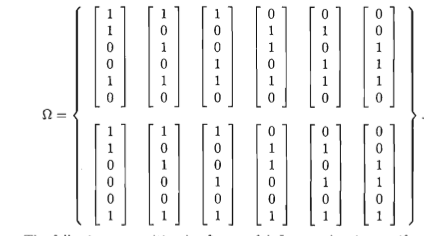
\includegraphics[height=1.5in]{omega.png}
			\label{fig:omega}
		\end{figure}		
	\end{frame}

	\begin{frame}{Causal Effects without assuming SUTVA}
		\begin{itemize}
			\item Without SUTVA, a causal effect is defined for every possible combination of the treatment assignment.
			\item The potential outcome for unit $i$ might be $Y_{i100000000000}$ or $Y_{i010000000000}$, etc. 
			\item How many potential outcomes will each unit have in a sample with $N$ observation? \pause 
			\textcolor{blue}{$2^N$} 
			\item Potential outcomes are still well defined when SUTVA is not satisfied! 
		\end{itemize}
	\end{frame}

\begin{frame}[t]\frametitle{SUTVA: Rubin (1986) \\ \small 
Statistics and Causal Inference: Comment: Which If's Have Causal Answers}
		\begin{itemize}
			\item<+-> In a comment to Holland (1986) Rubin provides a formal definition of SUTVA.
			\item<+-> There are $N$ units indexed by $u = 1,\dots,N$, $T$ treatments indexed by $t = 1,\dots,T$, and an outcome variable $Y_{tu}$
			\item<+-> Rubin's definition: \textit{"SUTVA is simply the a priori assumption that
the value of $Y$ for unit $u$ when exposed to treatment $t$ will
be the same no matter what mechanism is used to assign
treatment $t$ to unit $u$ and no matter what treatments the
other units receive" $\forall_t, \forall_u$}
		\item<+-> Examples when SUTVA is violated:
		\begin{enumerate}
		\item There exist unrepresented versions of treatments: \emph{$Y$ depends on which version of treatment $t$ was received}
		\item interference between units: \emph{the outcome, $Y$, of unit $u$ depends on whether
unit $u'$ received treatment $t$ or $t'$}
        \end{enumerate}		 
		\end{itemize}
	\end{frame}

\begin{frame}[t]\frametitle{SUTVA: Rubin (1986) \\ \small 
Statistics and Causal Inference: Comment: Which If's Have Causal Answers}
		\begin{itemize}
			\item Does the following statement has a causal meaning?\\
			\textit{If the females at firm $f$ had been male, their 
starting salaries would have averaged $20\%$ higher}\\ \pause
			 \textcolor{blue}{\textit{No, the statement is causal meaningless}}			 
			\item Rubin's answer: \\ \pause
			\emph{"the statement, by itself, is too
vague to have a clear formulation satisfying SUTVA and
thus is too vague to admit a clear causal answer. What are
the units, treatments, and outcomes such that SUTVA is
satisfied? I am not at all sure how to define anything except
$Y$, which clearly involves starting salary"} \pause
		\item See Rubin (1986) for a variety of ways to make the statement have a causal meaning 
		\end{itemize}
	\end{frame}


\begin{frame}{SUTVA: Example}
\begin{itemize}
\item Assume the following DGP (data generating process):
\[ Y_i =\alpha+\tau T_i +X_i \beta + \epsilon_i \]
\item Is SUTVA satisfied in this model? \pause \textcolor{blue}{Yes}
\item If $Cov(X_i,\epsilon_i)\neq 0$, $X_i$ is endogenous. Is SUTVA satisfied? \pause \textcolor{blue}{Yes}
\end{itemize}
\end{frame}

%%%%%%%%%%%%%%%%%%%%%%%%%%%%%%%%%%%%%%%%%%%%%%%
% End SUTVA, start CIA
%%%%%%%%%%%%%%%%%%%%%%%%%%%%%%%%%%%%%%%%%%%%%%%

\begin{frame}
\begin{itemize}
\item Consider the following model of the treatment effect (multiplicative treatment effect)
$$ Y_{i1} = \tau Y_{i0} $$
\item What is the $ATE$ effect?\\ \pause
\textcolor{blue}{Answer: $\mathbb{E}(Y_{i1} - Y_{i0}) = \mathbb{E}(\tau Y_{i0} - Y_{i0}) 
= \mathbb{E}(Y_{i0})(\tau -1)$} \pause
\item How can we estimate $\tau$? \pause 
\item One solution is to employ the following transformation on the data, $log$:
$$ log(Y_{i1}) = \tau+log(Y_{i0})$$
\pause
\item Now $\tau$ is the $ATE$ of the treatment after the transformation, and can be estimated by the difference in means
\end{itemize}
\end{frame}

\begin{frame}
\begin{itemize}
\item Prior to the $log$ transformation, what is the variance of the potential outcomes with the treatment? Is it equal to the variance under control?\pause
$$ \mathbb{V}(Y_{i1}) = \tau^2 \mathbb{V}(Y_{i0})$$ 
\pause
\item After the $log$ transformation, the variance in both groups is the same,
$$ \mathbb{V}(Y_{i1}) = \mathbb{V}(Y_{i0}+\tau)=\mathbb{V}(Y_{i0})$$ 
\end{itemize}
\end{frame}


\begin{frame}{Conditional independence assumption (CIA)}
\begin{itemize}
\item The CIA implies that:
$$ \mathbb{E}\left(Y_{i1}|X_i,T_i=1 \right) = \mathbb{E}\left(Y_{i1}|X_i,T_i=0 \right)
 = \mathbb{E}\left(Y_{i1}|X_i\right)$$
and 
$$ \mathbb{E}\left(Y_{i0}|X_i,T_i=1 \right) = \mathbb{E}\left(Y_{i0}|X_i,T_i=0 \right)
 = \mathbb{E}\left(Y_{i0}|X_i\right)$$
\pause
\item Assuming CIA holds, 
$$ATE =
 \mathbb{E}_{X_i}\left( \mathbb{E}_{Y_{i1}|X_i} \left(Y_{i1}|X_i,T_i=1 \right) \right)
 - \mathbb{E}_{X_i}\left( \mathbb{E}_{Y_{i0}|X_i} \left(Y_{i0}|X_i,T_i=0 \right) \right) $$
\end{itemize}
\end{frame}

\begin{frame}{Conditional assumption (CIA)}
\begin{itemize}
\item Assuming the following model (linear regression),
$$y_i = \alpha + \tau_1 T_i + X_i \beta +\epsilon$$ 
\pause
\item Then, 
$$\mathbb{E}(Y_i|T_i=1,X_i) = \alpha + \tau_1 + X_i \beta,\;\;  \mathbb{E}(Y_i|T_i=0,X_i) = \alpha + X_i \beta$$
\pause
\item In a regression model the standard assumption is that $X_i$ is fixed (not a random variable), and therefore,
$$ \mathbb{E}_{X_i}\left( \mathbb{E}_{Y_{i1}|X_i} \left(Y_{i1}|X_i,T_i=1 \right) \right) 
= \mathbb{E}_{Y_{i1}|X_i} \left(Y_{i1}|X_i,T_i=1 \right)$$
\pause
\item Therefore the parameter $\tau_1$ can be estimated by a regression adjustment, $\hat{\beta}_{OLS}^T$ 
\item There are also many other ways of estimating $\tau_1$, such as matching 
\end{itemize}
\end{frame}

\begin{frame}{Treatment assignment mechanisms}
\begin{itemize}
\item There are many possible random treatment assignment mechanisms. The must common is selecting $m$ observations to be assigned treatment out of $N$ possible units \\~\\ 

\item In this approach, $m$, is fixed, it is not a random variable. The source of randomization is the random assignment of treatment
\end{itemize}
\end{frame}

\begin{frame}{Treatment assignment mechanisms}
\begin{figure}
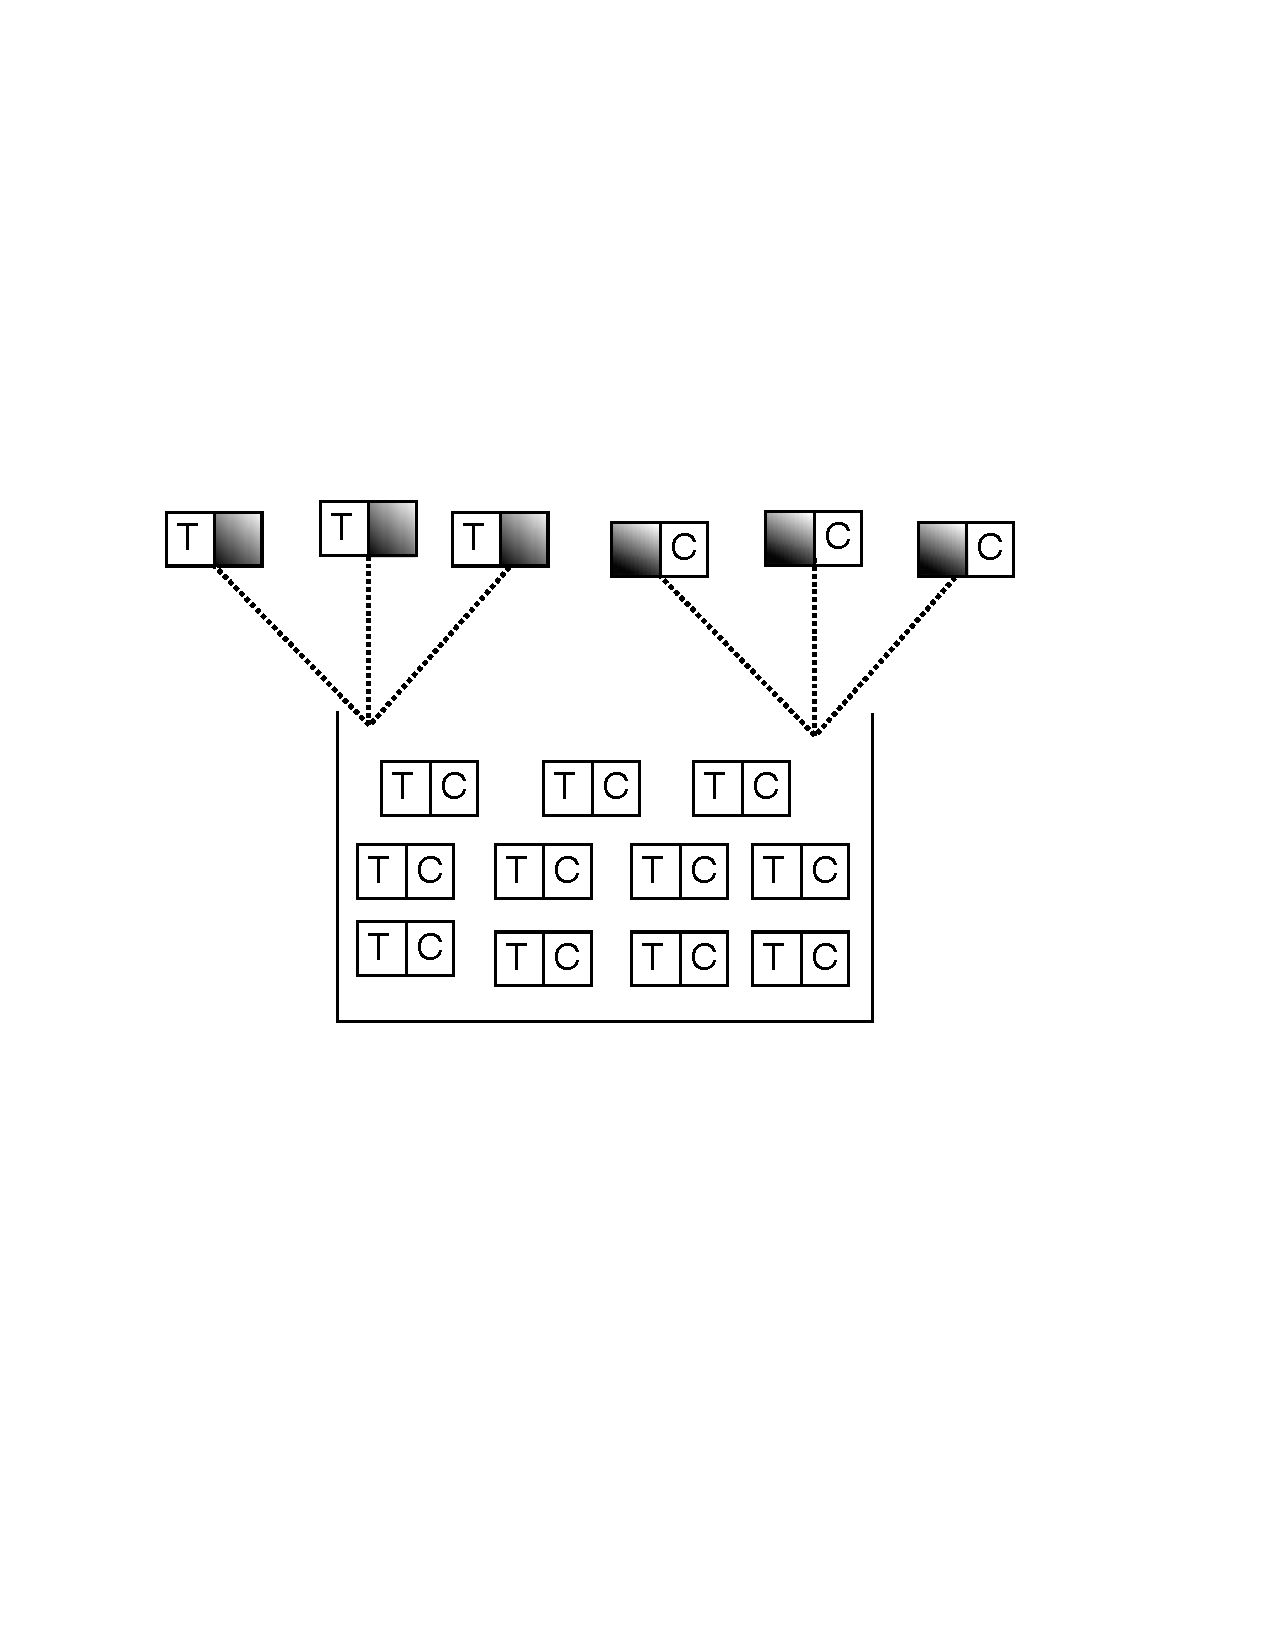
\includegraphics[scale=0.65]{potential_outcomes1.pdf}
\end{figure}
\end{frame}

\begin{frame}{Treatment assignment mechanisms}
\begin{itemize}
\item There are $N$ units, and $m$ units are assigned a binary treatment at random
\item Let $Z_i$ be an indicator variable whether unit $i$ was assigned treatment or control 
\item Is $Z_i$ and $Z_j$ independent? \pause \textcolor{blue}{\textit{No}}
\item What is $Cov(Z_i,Z_j)=?$ Is it positive or negative? \pause \textcolor{blue}{\textit{$Cov(Z_i,Z_j)<0$}, If unit $i$ is assigned treatment the probability of unit $j$ to receive treatment decreases. There is a negative relationship} 
\end{itemize}
\end{frame}

\begin{frame}{Treatment assignment mechanisms}
\begin{itemize}
\item What is, $Pr(Z_i=1|m)$? \pause \textcolor{blue}{$Pr(Z_i=1|m) = \frac{m}{N}$}
\item Is $Z_i$ and $Z_j$ independent? What is $cov(Z_i,Z_j)$? \pause
\item When there are $m$ units to be assigned treatment among $N$ remaining units, the probability of $Z_i=1$ conditional on $Z_j$ is? \\ \pause 
\textcolor{blue}{$Pr(Z_i=1|z_j=0) = \frac{m}{N-1}$,
 $Pr(Z_i=1|z_j=1) = \frac{m-1}{N-1}$}  
\item When $N\rightarrow\infty$: $Pr(Z_i=1|z_j=1)=Pr(Z_i=1|z_j=0)=Pr(Z_i=1)$ 
\pause
\item When $N \rightarrow \infty$, $Z_i$ and $Z_j$ are independent and $cov(Z_i,Z_j)=0$
\end{itemize}
\end{frame}


\begin{frame}{Calculating $Cov(Z_i,Z_j)$ Analytically}
As $Z_i$ is an indicator variable it follows that,
$$ \mathbb{E}(Z_i) = Pr(Z_i=1)=\frac{m}{N},\; \forall_i,j$$
\pause
$$ \mathbb{E}(Z_i \cdot Z_j) = 0\times 0 \times Pr(Z_i=0, Z_j=0)+ 1\times 0 \times Pr(Z_i=1, Z_j=0)+$$
$$ 0\times 1 \times Pr(Z_i=0, Z_j=1)+1\times 1 \times Pr(Z_i=1, Z_j=1)$$
\pause
$$ = Pr(Z_i=1, Z_j=1) = \frac{m}{N}\cdot \frac{m-1}{N-1}$$
Hence,\pause
$$Cov(Z_i,Z_j) = \mathbb{E}(Z_i \cdot Z_j) - \mathbb{E}(Z_i) \cdot \mathbb{E}(Z_j)$$
$$ = \frac{m}{N} \left(  \frac{m-1}{N-1} - \frac{m}{N} \right) < 0$$
\end{frame}

\begin{frame}{Monte Carlo simulations}
\begin{itemize}
\item An alternative approach for estimating $Cov(Z_i,Z_j)$ is by a Monte-Carlo approximation \pause \\~\\
\item The data generating process is known, a treatment was assigned at random, $m$ units where chosen out of $N$. We can construct a simulation which performs exactly this process a multiple number of time and using the repetitions approximate the random component of the assignment mechanism.   
\end{itemize}
\end{frame}

\begin{frame}[fragile]{Monte Carlo simulations: code}
\small
\begin{verbatim}
m=4
R=10000 #or 500000
n.vec = c(c(5:20),seq(21,100,by=5)) # sample sizes, N
cov.real1 <- cov.approx1 <- rep(999,length(n.vec))
for (i in c(1:length(n.vec))){  
  N = n.vec[i]  
 ## analytical: 
 cov.real1[i] <- (m/N)*((m-1)/(N-1)-(m/N))
 ### Simulation:
  z1<-z2<-rep(999,R)
  for (j in c(1:R)){
    id.treat = sample(c(1:N),m,replace=FALSE)
    treat0 = rep(0,N)
    treat0[id.treat]=1
    z1[j] = treat0[1]
    z2[j] = treat0[2]
  } 
  cov.approx1[i] <- cov(z1,z2)
}
\end{verbatim}
\normalsize
\end{frame}

\begin{frame}{Monte Carlo simulations: Results}
\begin{figure}
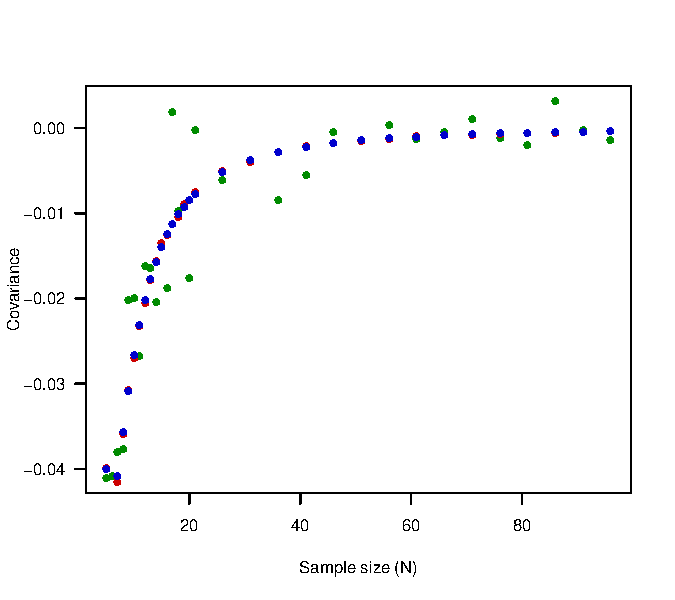
\includegraphics[scale=0.8]{figure_cov.pdf}
\end{figure}
\end{frame}




\end{document}



















\end{document}